% \iffalse meta-comment
%
% Copyright (C) 2023 by Kushagra Lakhwani <korigamik@gmail.com>
% -------------------------------------------------------

%<*internal>
\iffalse
%</internal>

%<*internal>
\fi
\def\nameofplainTeX{plain}
\ifx\fmtname\nameofplainTeX\else
  \expandafter\begingroup
\fi
%</internal>

%<*install>
\input docstrip.tex
\keepsilent
\askforoverwritefalse
\preamble
---------:| ----------------------------------------------------------
korigamik:| KorigamiK LaTeX Template
   Author:| Kushagra Lakhwani
   E-mail:| korigamik@gmail.com
  License:| Released under the GNU General Public License v3 or later
      See:| http://www.gnu.org/licenses/
\endpreamble

\postamble

Copyright (C) 2023 by Kushagra Lakhwani <korigamik@gmail.com>

KorigamiK class is free software: you can redistribute it and/or modify
it under the terms of the GNU General Public License as published by
the Free Software Foundation, either version 3 of the License, or (at
your option) any later version.

KorigamiK class is distributed in the hope that it will be useful, but
WITHOUT ANY WARRANTY; without even the implied warranty of
MERCHANTABILITY or FITNESS FOR A PARTICULAR PURPOSE.  See the GNU
General Public License for more details.

You should have received a copy of the GNU General Public License
along with KorigamiK class.  If not, see <http://www.gnu.org/licenses/>.

\endpostamble

\usedir{tex/latex/korigamik}
\generate{
  \file{\jobname.cls}{\from{\jobname.dtx}{class}}
}

%</install>
%<install>\endbatchfile
%<*internal>
\usedir{source/latex/korigamik}
\generate{
  \file{\jobname.ins}{\from{\jobname.dtx}{install}}
}
\nopreamble\nopostamble
\ifx\fmtname\nameofplainTeX
  \expandafter\endbatchfile
\else
  \expandafter\endgroup
\fi
%</internal>
% \fi
%
% \iffalse
%<*driver>
\ProvidesFile{korigamik.dtx}
%</driver>
%<class>\NeedsTeXFormat{LaTeX2e}[1999/12/01]
%<class>\ProvidesClass{korigamik}
%<*class>
    [2023/06/24 v1.10 KorigamiK LaTeX Template]
%</class>
%<*driver>
\documentclass{ltxdoc}
\usepackage[a4paper,margin=25mm,left=50mm,nohead]{geometry}
\usepackage[numbered]{hypdoc}
\EnableCrossrefs
\CodelineIndex
\RecordChanges
\begin{document}
  \DocInput{\jobname.dtx}
\end{document}
%</driver>
% \fi
%
% \GetFileInfo{\jobname.dtx}
% \DoNotIndex{\newcommand,\newenvironment}
%
%\title{The \textsf{korigamik} class \thanks{This file
%   describes version \fileversion, last revised \filedate.}
%}
%\author{Kushagra Lakhwani\thanks{E-mail: korigamik@gmail.com}}
%
%\maketitle
%
%\changes{v1.00}{2023/03/27}{First public release}
%\changes{v1.10}{2023/06/24}{Added documentation and fixed bugs}
%
% \begin{abstract}
%   The \textsf{KorigamiK} class is used for typesetting documents for university or 
%   school projects and lab reports. It is based on the article class with 
%   modifications to allow for more flexible front-matter among other changes.
% \end{abstract}
%
% \section{Usage}
%
% ==== Put descriptive text here. ====
%
% \DescribeMacro{\dummyMacro}
% This macro does nothing.\index{doing nothing|usage} It is merely an
% example.  If this were a real macro, you would put a paragraph here
% describing what the macro is supposed to do, what its mandatory and
% optional arguments are, and so forth.
%
% \DescribeEnv{dummyEnv}
% This environment does nothing.  It is merely an example.
% If this were a real environment, you would put a paragraph here
% describing what the environment is supposed to do, what its
% mandatory and optional arguments are, and so forth.
%
%\StopEventually{
%  \PrintChanges
%  \PrintIndex
%}

% \section{Implementation}
% The implementation of the \textsf{korigamik} class is given below.
%
%
% \textbf{Derive your class from the \textsf{article} class.}
%    \begin{macrocode}
\LoadClass[12pt]{article}
\RequirePackage[a4paper,margin=1in,tmargin=1.5in]{geometry}
%    \end{macrocode}

% \textbf{Required packages}
%    \begin{macrocode}
\RequirePackage{tikz,color,hyperref,graphicx}
\usetikzlibrary{positioning,calc}
%    \end{macrocode}

% \textbf{Font settings}
%    \begin{macrocode}
\RequirePackage[T1]{fontenc}
\RequirePackage{lmodern} % modernized version of the Computer Modern font family  
\RequirePackage[sc]{mathpazo} % small caps option (sc) 
\RequirePackage{textcomp} % provides additional symbols and text companion fonts.
\RequirePackage[protrusion=true,expansion=false]{microtype} % enabling character protrusion) (disabling font expansion)
%    \end{macrocode}

% \textbf{Page layout}
%    \begin{macrocode}
\RequirePackage{fancyhdr}
\fancypagestyle{firstpage}{%
	\fancyhf{} % clear all six fields
	\renewcommand{\headrulewidth}{0pt}
	\renewcommand{\footrulewidth}{0pt}
}
\fancypagestyle{followingpage}{
	\fancyhf{} % clear all six fields
	\fancyhead[LO, L]{\@header}
	\fancyhead[RO]{\nouppercase\leftmark}
	\fancyhead[R]{\nouppercase\leftmark}
	\setlength{\headheight}{15pt}
	\fancyfoot{}
	\fancyfoot[L,LO]{\hfill\thepage\hfill}
}

\pagestyle{followingpage}
\AtBeginDocument{\thispagestyle{firstpage}}
\linespread{1.069}
%    \end{macrocode}

% \begin{macro}{\linkcolour}
% This macro defines the colour of the hyperlinks.
%    \begin{macrocode}
\definecolor{linkcolour}{rgb}{0.286,0.286,0.286}
%    \end{macrocode}
% \end{macro}

% \textbf{Configurations}
%    \begin{macrocode}
\newcommand*{\@rollno}{<rollno>}
\newcommand*{\rollno}[1]{	\renewcommand*{\@rollno}{#1} }
\newcommand*{\@subject}{<subject>}
\newcommand*{\subject}[1]{ \renewcommand*{\@subject}{#1} }
\newcommand*{\@keywords}{<keywords>}
\newcommand*{\keywords}[1]{	\renewcommand*{\@keywords}{#1} }
\newcommand*{\@logoimagepath}{}
\newcommand*{\@logoimagescale}{0.5}
\newcommand*{\@logolabel}{<Logo label>}
\newcommand*{\logoimage}[3]{  \renewcommand*{\@logoimagepath}{#1}
                              \renewcommand*{\@logoimagescale}{#2}
                              \renewcommand*{\@logolabel}{#3} }
\newcommand*{\@titlelabel}{<Something here>}
\newcommand*{\titlelabel}[1]{ \renewcommand*{\@titlelabel}{#1} }
\newcommand*{\@semester}{<semester>}
\newcommand*{\semester}[1]{	\renewcommand*{\@semester}{#1} }
\newcommand*{\@header}{<header>}
\newcommand*{\header}[1]{	\renewcommand*{\@header}{#1} }
\newcommand*{\@bottomnote}{<bottom note>}
\newcommand*{\bottomnote}[1]{	\renewcommand*{\@bottomnote}{#1} }
\newcommand*{\@course}{<course>}
\newcommand*{\course}[1]{	\renewcommand*{\@course}{#1} }
%    \end{macrocode}

% \textbf{Hyperref settings}
%    \begin{macrocode}
\hypersetup{  colorlinks,breaklinks,
  linkcolor=linkcolour,citecolor=linkcolour,
  filecolor=linkcolour, urlcolor=linkcolour,
  pdftitle={\@title}, pdfauthor={\@author}
  pdfsubject={\@subject}, pdfkeywords={\@keywords}, }
%    \end{macrocode}

% \begin{macro}{\square}
% This is a macro that draws a square.
%    \begin{macrocode}
\newcommand{\square}{
	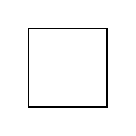
\begin{tikzpicture}
		\draw (0,0) -- (1,0) -- (1,1) -- (0,1) -- (0,0);
	\end{tikzpicture}
}
%    \end{macrocode}
% \end{macro}

% \begin{macro}{\maketitle}
% This is the macro that actually typesets the title page.
%    \begin{macrocode}
\renewcommand{\maketitle}{%
	\newgeometry{tmargin=1in,bmargin=.5in}
	\makeatletter
	\begin{titlepage}
		\begin{center}
			\begin{flushright}
				\ifx\@logoimagepath\empty
					\square
					\\<your logo here>
				\else
					\includegraphics[scale=\@logoimagescale]{\@logoimagepath}
					\Large {\\ \textbf{\@logolabel}}
				\fi
			\end{flushright}
		\end{center}
		\vfill

		\noindent\begin{tikzpicture}
			\node[
				text width=\textwidth-2cm,
				align=left,
				font=\fontsize{30}{30}\selectfont\scshape,
				inner xsep=.5cm
			] (x) {\@title};
			\draw (x.north west) node[
				draw,
				above right=1cm and 0pt,
				font=\LARGE,
				inner sep=.2cm
			] (y) {\textsc{\@titlelabel}};
			\draw (y.south west)--($(x.south west)+(0,-1)$);
		\end{tikzpicture}

		\vspace*{2cm}
		\begin{center}
			\begin{minipage}{\textwidth}
				\begin{tabular}[h]{l  l}
					Name     & \textbf{\@author}          \\
					\ifx\@rollno\empty
					\else
					Roll No. & \textbf{\textit{\@rollno}} \\
					\fi
					\ifx\@semester\empty
					\else
					Semester & \textbf{\@semester}        \\
					\fi
					\ifx\@course\empty
					\else
					Course   & \textbf{\textit{\@course}} \\
					\fi
				\end{tabular}
			\end{minipage}
		\end{center}
		\vfill

		\begin{center}
			\textsc{\large \@bottomnote}\\[0.4cm]
			{\large \today}
		\end{center}

	\end{titlepage}
	\makeatother
	\restoregeometry
}
%    \end{macrocode}
% \end{macro}

% \textbf{Define new sectioning commands}
%    \begin{macrocode}
\renewcommand\section{\@startsection {section}{1}{\z@}%
  {-3.5ex \@plus -1ex \@minus -.2ex}%
  {2.3ex \@plus.2ex}%
  {\normalfont\Large\raggedright}}
\renewcommand\subsection{\@startsection{subsection}{2}{\z@}%
	{-3.25ex\@plus -1ex \@minus -.2ex}%
	{1.5ex \@plus .2ex}%
	{\normalfont\large\raggedright}}
\renewcommand\subsubsection{\@startsection{subsubsection}{3}{\z@}%
	{-3.25ex\@plus -1ex \@minus -.2ex}%
	{1.5ex \@plus .2ex}%
	{\normalfont\normalsize\raggedright}}
\renewcommand\paragraph{\@startsection{paragraph}{4}{\z@}%
	{3.25ex \@plus1ex \@minus.2ex}%
	{-1em}%
	{\normalfont\normalsize\itshape}}
\renewcommand\subparagraph{\@startsection{subparagraph}{5}{\parindent}%
	{3.25ex \@plus1ex \@minus .2ex}%
	{-1em}%
	{\normalfont\normalsize\itshape}}

\newcommand\tpj@deflogo{\@dblarg\tpj@@deflogo}

\newcommand\tpj@@deflogo[3][\@nil]{%
	\expandafter\DeclareRobustCommand\csname#2\endcsname{#3}%
	\pdfstringdefDisableCommands{%
		\expandafter\def\csname#2\endcsname{#1}}}
%    \end{macrocode}

% \textbf{Define some logos}
%    \begin{macrocode}
\makeatletter
\tpj@deflogo{TeX}{T\kern-.15em\lower.5ex\hbox{E}\kern-.07em X\spacefactor1000\relax}
\tpj@deflogo{LaTeX}{L\kern-.32em\raise.37ex\hbox{\scalebox{0.76}{A}}\kern-.15em\TeX}
\tpj@deflogo{LaTeXe}{\LaTeX2$_{\textstyle\varepsilon}$}
\tpj@deflogo{BibTeX}{B{\textsc i\kern-.025em\textsc b}\kern-.08em\TeX}
\DeclareRobustCommand\logofamily{%
	\not@math@alphabet\logofamily\relax
	\fontencoding{U}\fontfamily{logo}\selectfont}
\DeclareTextFontCommand{\textlogo}{\logofamily}
\tpj@deflogo[MetaFont]{MF}{\textlogo{META}\@dischyph\textlogo{FONT}\@}
\tpj@deflogo[MetaPost]{MP}{\textlogo{META}\@dischyph\textlogo{POST}\@}
\tpj@deflogo{ConTeXt}{C\kern-.03em on\-\kern-.10em\TeX\kern-0.04em t}%
\tpj@deflogo{pdfTeX}{pdf\/\TeX}
\tpj@deflogo{pdfLaTeX}{pdf\/\LaTeX}
\makeatother
%    \end{macrocode}


% \textbf{Lists}
%
% Save the original itemize, enumerate, and description environments
%    \begin{macrocode}
\let\originalItemize\itemize
\let\originalEndItemize\enditemize
\let\originalEnumerate\enumerate
\let\originalEndEnumerate\endenumerate
\let\originalDescription\description
\let\originalEndDescription\enddescription
%    \end{macrocode}

% Redefine the itemize environment
%    \begin{macrocode}
\renewenvironment{itemize}
{\originalItemize\parskip=0pt}
{\originalEndItemize}
%    \end{macrocode}

% Redefine the enumerate environment
%    \begin{macrocode}
\renewenvironment{enumerate}
{\originalEnumerate\parskip=0pt}
{\originalEndEnumerate}
%    \end{macrocode}

% Redefine the description environment
%    \begin{macrocode}
\renewenvironment{description}
{\originalDescription\parskip=0pt\parindent=1.8em}
{\originalEndDescription}
%    \end{macrocode}

% Define aliases for itemize and enditemize
%    \begin{macrocode}
\let\itemise\itemize
\let\enditemise\enditemize
%    \end{macrocode}

% Redefine the label for the first level of itemize 
%    \begin{macrocode} 
\renewcommand\labelitemi{\normalfont\bfseries\textendash}
%    \end{macrocode}

% Redefine the label for the second level of itemize
%    \begin{macrocode} 
\renewcommand\labelitemii{\normalfont\bfseries\textperiodcentered}
%    \end{macrocode}

% Redefine the label for the description environment
%    \begin{macrocode} 
\renewcommand*\descriptionlabel[1]{\hspace\labelsep
	\normalfont\itshape #1}
%    \end{macrocode}

% Table of Contents
%    \begin{macrocode} 
\renewcommand*\contentsname{\centering \Huge Index \vskip 1cm}
\setcounter{tocdepth}{3} % Set the depth of the table of contents
%    \end{macrocode}

%
%    \begin{macrocode}
\endinput
%    \end{macrocode}

%\Finale
